\chapter{Aplikácie pre platformu Android}
\section{Android Application Package}
Aplikácie pre platformu Android sú vyvíjané predovšetkým v jazyku Java, ich vývoj je však možný aj v jazykoch C++, Kotlin, Python, alebo prostredníctvom technológie Xamarin ktorá využíva jazyk C\#. Výstupom kompilácie a zabalenia Android aplikácie je súbor typu Android Application Package. Tento súbor slúži ako inštalačný balíček, ktorý je pomocou distribučných kanálov distribuovaný k cieľovým užívateľom.

Android Application Package, skrátene APK, je formát archívnych súborov. APK súbory sú asociované s MIME typom \zv{application/vnd.android.package-archive} a príponou \zv{.apk}~\cite{IANA}. 

Formát APK súborov rozširuje JAR formát. Obidva spomínané formáty vychádzajú z archívneho formátu ZIP. Vďaka tejto vlastnosti je možné obsah archívu extrahovať pomocou štandardných nástrojov pre prácu so súbormi vo formáte ZIP.

APK súbory vznikajú ako výstup kompletnej kompilácie a zabalenia aplikácie. APK archív obsahuje súbory potrebné pre spustenie aplikácie. Typický obsah balíčka tvoria nasledujúce typy súborov:
\begin{itemize}
	\item skompilovaný zdrojový kód aplikácie
	\item súbor Manifest – súbor obsahujúci metadáta o danej aplikácií
	\item XML súbory – súbory definujúce rozloženie užívateľského rozhrania a konštantné hodnoty využívané aplikáciu, napr. definície farieb alebo textov
	\item multimediálne zdrojové súbory~\cite{Allen2015}.
\end{itemize}

\subsection{Štruktúra}
APK súbory dodržiavajú presne stanovenú vnútornú štruktúru. Táto štruktúra je znázornená na obrázku \ref{fig:strukturaApk}.

\begin{figure}[htb]
  \begin{center}
    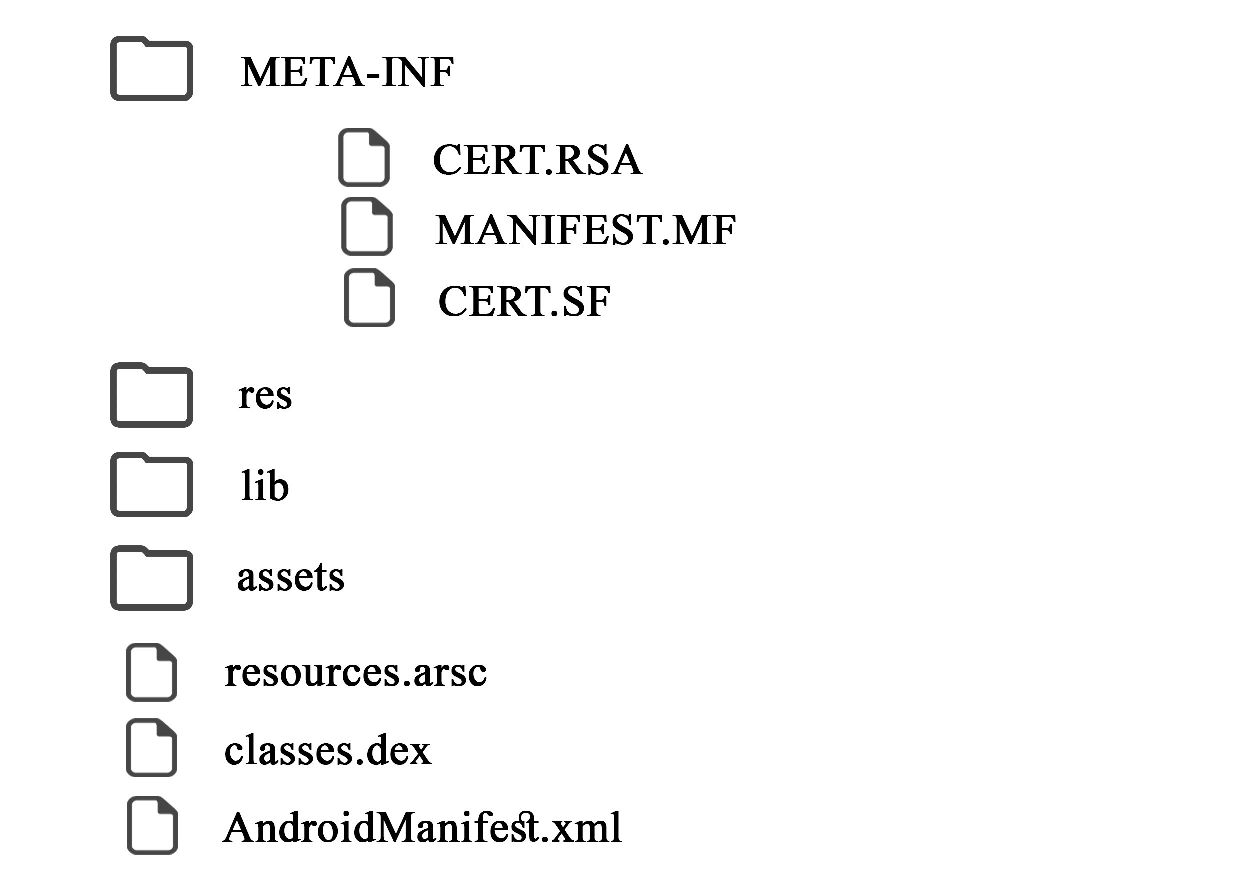
\includegraphics[width=60mm]{images/apkStructure.pdf}
  \end{center}
  \caption{Typická štruktúra APK súboru}
  \label{fig:strukturaApk}
\end{figure}


V APK súbore nájdeme nasledujúce súbory a adresáre:
\begin{itemize}

	\item \bod{AndroidManifest.xml} -- súbor obsahujúci meta informácie o aplikácii. Pomocou tohto súboru oznamuje aplikácia operačnému systému svoju identitu a požiadavky. Android Manifest sa v APK balíčku nachádza vo formáte skompilovaného binárneho XML.
Súbor AndroidManifest.xml obsahuje okrem iného informácie o nasledujúcich vlastnostiach aplikácie:
		
		\begin{itemize}
			\item meno balíku aplikácie slúžiace ako unikátny identifikátor aplikácie,
			\item najnižšiu verziu Android API na ktorej je aplikácia spustiteľná
			\item popisuje základné komponenty aplikácie, obsahuje informácie o aktivitách, službách (service), poskytovateľoch obsahu (content provider), prijímačoch (broadcast receiver) a triedach ktoré ich v rámci aplikácie implementujú,
			\item deklaruje povolenia vyžadované aplikáciou na prístup k zabezpečeným častiam Android API,
			\item definuje povolenia vyžadované od iných aplikácií pri interakcii s danou aplikáciou~\cite{Manifest}.
		\end{itemize}
	
	\item \bod{Classes.dex} -- súbor obsahujúci spustiteľný kód aplikácie. Súbor typu DEX (Dalvik Executable) obsahuje operačné kódy a inštrukcie špecifické pre behové prostredie Android Runtime a virtuálny stroj Dalvik Virtual Machine (pre verzie Android 4.4.4 a staršie)~\cite{DexFormat}. 

	\item \bod{Resources.arsc} -- tento súbor obsahuje informácie o zdrojových súboroch aplikácie. Tento súbor určuje vzťah medzi zdrojovými súbormi a ich identifikátormi, pomocou ktorých sú súbory referencované v zdrojovom kóde aplikácie.
	
	\item \bod{Assets} -- adresár obsahujúci neskomprimované zdrojové súbory.  Na rozdiel od zdrojových súborov z priečinku res, tieto zdroje nie sú referencované identifikátorom, ale prístup k nim je umožnený pomocou API triedy AssetManager.
	
	\item \bod{Lib} -- v tomto adresári sa nachádzajú skompilované knižnice určené pre konkrétnu architektúru procesora. Medzi podporované architektúry patrí ARMv7 a novšie, x86, x86\_64.

	\item \bod{Res} -- adresár obsahujúci zdroje aplikácie. Obsah tohto adresára je tvorený predovšetkým multimediálnymi súbormi ako napríklad obrázky a ikony, ale aj súbormi vo formáte XML ktoré definujú užívateľské rozhranie, farby, lokalizované texty alebo štýl aplikácie. Súbory umiestnené v tomto adresári sú v zdrojovom kóde referencované pomocou unikátnych číselných identifikátorov, ktoré sú vygenerovaný počas kompilácie a nachádzajú sa v triede \zv{R.java}. Obsah priečinku je ďalej logicky členený do viacerých podpriečinkov. Android podporuje lokalizáciu a rôzne verzie zdrojových súborov, ktoré použije na základe údajov o zariadení na ktorom je aplikácia spustená~\cite{Resources}.
	
	\item \bod{META-INF} -- v tomto adresári sa nachádzajú súbory zaručujúce digitálny podpis a integritu APK balíčku. 
		\begin{itemize}
			\item CERT.RSA  -- súbor obsahujúci certifikát podpisu aplikácie
			\item MANIFEST.MF  -- súbor obsahujúci hash každého súboru v APK archíve. Využíva hashovaciu funkciu \zv{SHA-1}.
			\item CERT.SF  -- súbor obsahujúci záznam o každom súbore v APK archíve. Záznam o jednom súbore obsahuje jeho názov a \zv{SHA-1} hash záznamu o tomto súbore z MANIFEST.MF.
		\end{itemize}		
		
		
\end{itemize} 


\section{Distribúcia aplikácií}
Aplikácie na platforme Android sú distribuované ako inštalačné APK balíčky. 

Podľa formy distribúcie a inštalácie môžeme aplikácie rozdeliť na dve základné skupiny
\begin{itemize}
 \item \bod{Predinštalované (systémové) aplikácie} -- tieto aplikácie sú distribuované priamo so zariadením a sú nainštalované pri iniciálnom zapnutí zariadenia,
 \item \bod{Užívateľské aplikácie} -- aplikácie distribuované vo forme balíčkov poskytovaných najčastejšie pomocou obchodov s aplikáciami.
\end{itemize}

Zoznam predinštalovaných aplikácií určuje výrobca zariadenia. Používateľ nemá možnosť systémové aplikácie odinštalovať. Do kategórie predinštalovaných systémových aplikácií patria aplikácie umožňujúce ovládanie základného vybavenia zariadenia ako napríklad aplikácia telefón alebo fotoaparát. Do tejto kategórie patria aj predinštalované služby od spoločnosti Google. 

Užívateľské aplikácie slúžia na prispôsobenie systému pre potreby konkrétneho užívateľa. O inštalácií a odstránení užívateľských aplikácií rozhoduje používateľ. Na pohodlné prehliadanie a inštaláciu aplikácií slúžia obchody (app stores). Pomocou centralizovaných obchodov s aplikáciami môžu softvéroví vývojári jednoducho dostať svoju aplikáciu k veľkému počtu užívateľov.  Najrozšírenejším a najznámejším obchodom s aplikáciami pre platformu Android je oficiálny obchod 
\zv{Google Play Store}. 

Okrem oficiálneho obchodu sú aplikácie distribuované aj pomocou alternatívnych distribučných kanálov. Medzi takéto kanály zaraďujeme alternatívne obchody s aplikáciami ako napríklad \zv{Amazon Appstore}. Častým distribučným kanálom sú aj obchody výrobcov mobilných zariadení alebo obchody mobilných operátorov. Existuje viacero služieb tretích strán ktoré sprostredkovávajú prístup k oficiálnym aplikáciám z týchto obchodov. APK súbory sú distribuované aj pomocou warezových portálov na zdieľanie súborov alebo underground obchodov. 

Z dôvodu udržania bezpečného a spoľahlivého fungovania platformy Android je dôležitá bezpečnosť a kvalita distribuovaných aplikácií. Výskum porovnávajúci kvalitu aplikácií na neoficiálnych distribučných platformách ukázal, že tieto distribučné kanály obsahujú $5 až 13\%$ aplikácií, ktoré sú klonom oficiálnych aplikácií distribuovaných pomocou \zv{Google Play Store} ~\cite{Zhou2012}.

\section{Inštalácia aplikácií}

Platforma Android poskytuje služby na inštaláciu, aktualizáciu a odinštalovanie aplikácií. \newline
Základnú funkcionalitu poskytujú nasledujúce služby.
\begin{itemize}
	\item \bod{Package Installer} -- implementuje funkcionalitu inštalácie, aktualizácie a odinštalovania aplikácií,
	\item \bod{Package Manager Service} -- poskytuje API pre správu nainštalovaných softvérových balíčkov,
	\item \bod{Daemon Installd} -- vytvára a spravuje adresáre potrebné pre nainštalovanie aplikácie.
\end{itemize}
Inštalácia aplikácie pozostáva z overenia aplikácie a extrakcie dát z APK balíčka. Aplikácia je overená na základe digitálneho podpisu a metadát zo súboru \zv{AndroidManifest.xml}. Systémové aplikácie sú rozbalené do adresára \cesta{/system/app}. Užívateľské aplikácie sú nainštalované v adresári \cesta{/data/app}. Systém Android uchováva v spomínaných adresároch kompletné APK súbory~\cite{AndroidDeveloper}.


